\documentclass{sig-alternate-10pt}
\usepackage{amsfonts,xspace}
\usepackage{url}
\usepackage{epsfig}
\usepackage{graphicx}
\usepackage{subfigure}
\usepackage{ifpdf}
\usepackage[usenames,dvipsnames]{color}
\newcommand{\tbd}[1]{}
\newcommand{\ie}{{\it i.e.}}
\newcommand{\eg}{{\it e.g.}}
\newcommand{\etc}{{\it etc.}}
\newcommand{\eat}[1]{}
\usepackage[english,plain]{fancyref}
\usepackage{times}
\usepackage{rotating}
\usepackage[labelformat=simple]{subfig}


\newcommand{\mypara}[1]{\medskip\noindent{\bf {#1}:}~}
\newcommand{\chk}{$\checkmark$}
\newcommand{\dsh}{{\bf --}}
\newcommand{\til}{{\bf\large \textasciitilde}}
%\newcommand{\tbd}[1]{[{\color{red}{\bf{TBD: #1}}}]}
\newcommand{\etal}{\emph{et~al.}}
\newcommand{\meddle}{{Meddle}\xspace}
\newcommand{\dsum}{\displaystyle\sum}
\newcounter{packednmbr}

\newenvironment{packedenumerate}{\begin{list}{\thepackednmbr.}{\usecounter{packednmbr}\setlength{\itemsep}{0.2pt}\addtolength{\labelwidth}{-4pt}\setlength{\leftmargin}{\labelwidth}\setlength{\listparindent}{\parindent}\setlength{\parsep}{1pt}\setlength{\topsep}{0pt}}}{\end{list}}
\newenvironment{packeditemize}{\begin{list}{$\bullet$}{\setlength{\itemsep}{0.2pt}\addtolength{\labelwidth}{-4pt}\setlength{\leftmargin}{\labelwidth}\setlength{\listparindent}{\parindent}\setlength{\parsep}{1pt}\setlength{\topsep}{0pt}}}{\end{list}}
\newenvironment{packedtrivlist}{\begin{list}{\setlength{\itemsep}{0.2pt}\addtolength{\labelwidth}{-4pt}\setlength{\leftmargin}{\labelwidth}\setlength{\listparindent}{\parindent}\setlength{\parsep}{1pt}\setlength{\topsep}{0pt}}}{\end{list}}

\renewcommand{\fref}{\Fref}
\renewcommand\thesubfigure{~(\alph{subfigure})}

\title{\meddle: Middleboxes for Increased Transparency and Control of Mobile Traffic }
% middlebox transparency control mobile traffic 
\numberofauthors{6}
\author{
\alignauthor
Ashwin Rao\\
\affaddr{INRIA}
\alignauthor        
David Choffnes\\
\affaddr{University of Washington}
\alignauthor
Justine Sherry\\
\affaddr{UC Berkeley}
\and
\alignauthor
Arnaud Legaut\\
\affaddr{INRIA}
\alignauthor 
Arvind Krishnamurthy\\
\affaddr{University of Washington}
\alignauthor
Walid Dabbous\\
\affaddr{INRIA}
}



\date{}
\begin{document}	
\maketitle

\begin{abstract}
In this poster we present \meddle, a framework aimed at enhancing
the transparency in mobile networks and providing a platform that lets
users reclaim control over their mobile traffic. We argue that
\meddle, which builds upon VPN and middleboxes, is feasible to
implement, and is capable of  providing sufficient incentives for 
large scale experiments and user based measurement studies.    
\end{abstract}

\begin{keywords}
Middlebox, Mobile, VPN, Measurement platform.
\end{keywords}

\section{Introduction}

\meddle is motivated by the opaque nature of mobile systems and the
limited control users have over how their mobile devices use the
various networks they pay for. In the mobile environment, users are
forced to interact with a single operating system tied to their
device, generally use closed-source apps provided for the OS that
routinely violate user privacy~\cite{hornyack:appfence}, and subscribe
to network providers that can (and do) transparently modify, block or
otherwise interfere with network traffic~\cite{wang:middleboxes}. 

Researchers face a similar set of challenges for characterizing an
experiment for mobile systems. To characterize mobile traffic and
design new protocols and services that are better tailored to the
mobile environment, we would like a framework that allows us to
intercept and potentially modify traffic generated by mobile devices
as they move with users, regardless of the device, OS or
carrier. However, implementing this functionality is difficult on
mobile devices because it requires warranty-voiding techniques such as
jail breaking to access and manipulate traffic at the network
layer~\cite{enck:taintdroid}. Even when using such an approach,
carriers may manipulate traffic once it leaves the mobile
device~\cite{wang:middleboxes}, thus rendering some research
impractical. Last, some protocols and services should be implemented
in the network instead of the device (e.g., prefetching and security
filters) but researchers generally have no ability to deploy such
solutions.

In this poster, we show that \meddle provides the necessary
framework to simultaneously address these issues for users and
researchers. \meddle relies on VPN tunnels to route mobile traffic
through it. Once packets arrive at a \meddle server, we can use a
variety of middlebox approaches to transform traffic to and from
mobile devices. This enables new research in both measuring and
characterizing mobile traffic, and designing new in-network features
to improve the mobile experience. \meddle also enables researchers
to investigate what-if scenarios for the impact of new middleboxes as
if they were deployed in carrier networks.   

\eat{
  -- services for cell phones
        -- what's diff't about cell phones?
            -- power
                -- prefetching/batching data
                -- offloading processing (virus scanning, comp vision, data analysis)
            -- exfiltration/desire to monitor (even from user)
            -- device limitations (transcoding)
           
        -- what's slightly different but needs tweaked?
            -- IDS -- different attacks/viruses
            -- Proto accel -- some protocols difft?

        -- what's exactly the same
            -- performance
            -- privacy (Do not Track, obfuscation)
            -- Protocol rollout (DNSSEC; SPDY, MPTCP)

    -- users locked out of their own devices
    -- platform for measurement
        }
\eat{
    \section{Service Deployment}

    \section{Measurement Platform}

    \section{Challenges}

    \section{Conclusion \& Related Work}\
}
   
\section{\meddle Architecture}

\begin{figure}
  \centering
  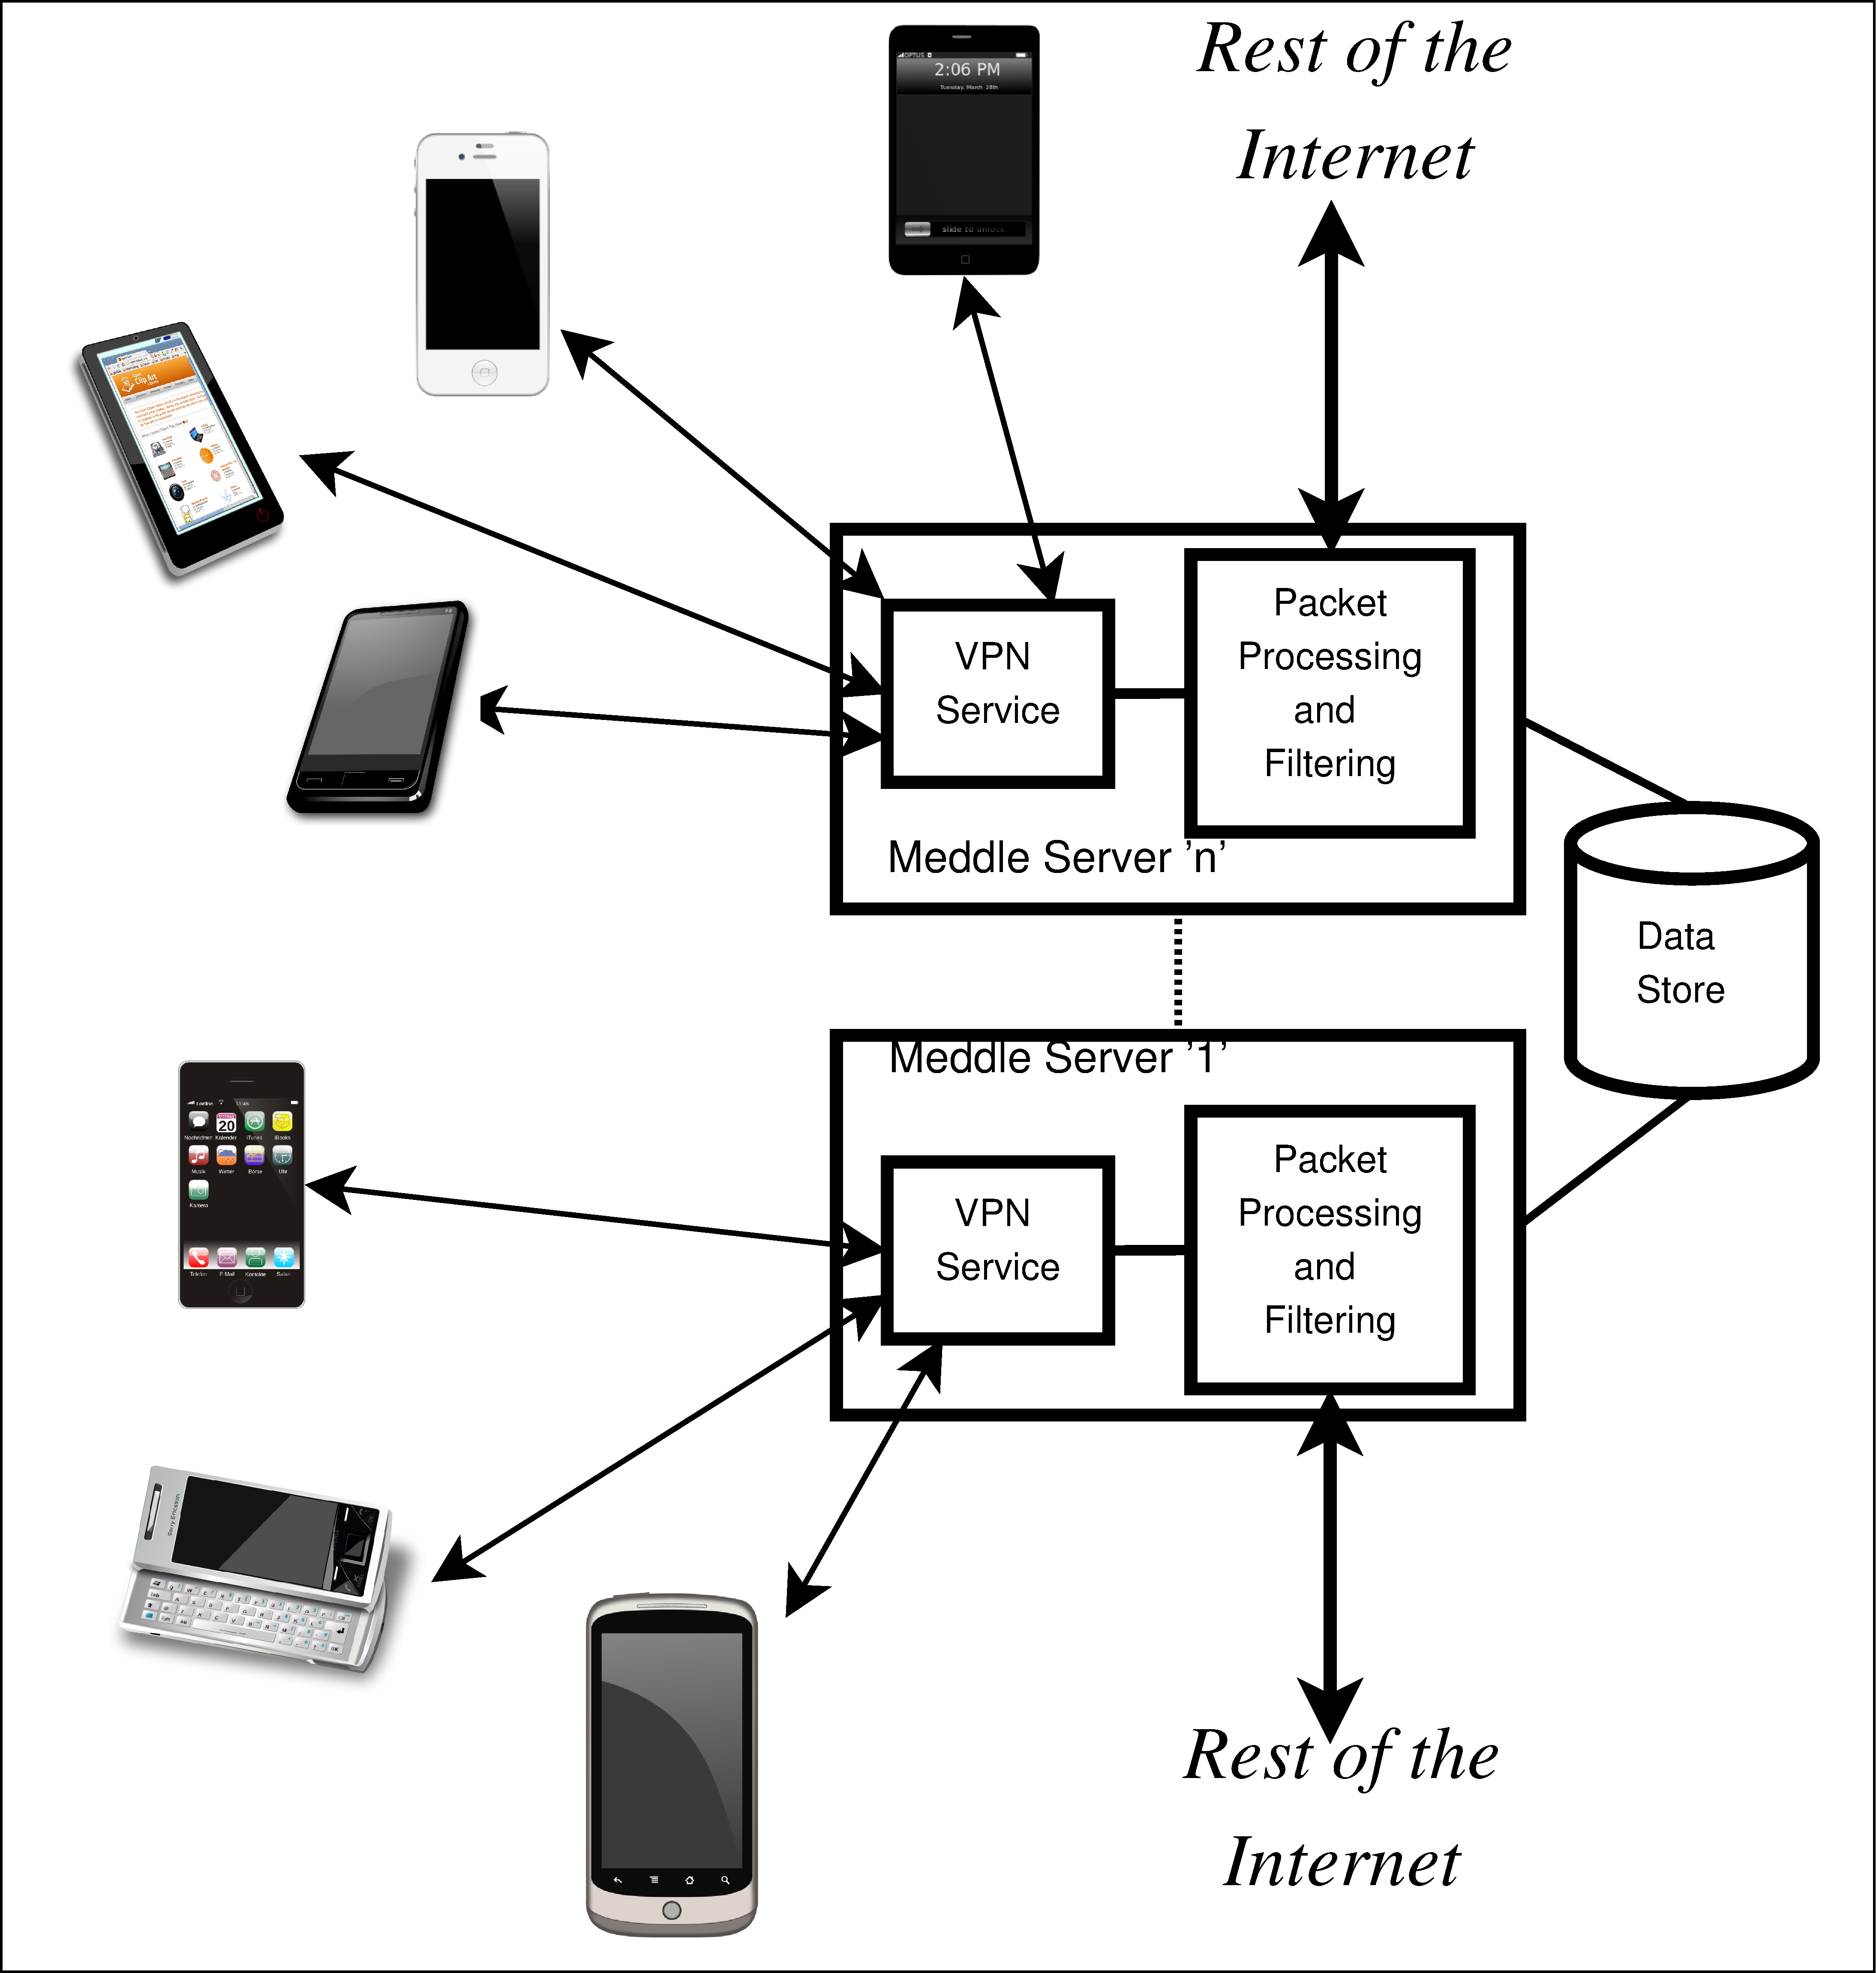
\includegraphics[width=0.6\columnwidth]{figures/meddle-servers.pdf}
  \caption{Meddle deployment. \emph{Clients connect to a \meddle
      server depending on their location. Client configurations are
      stored in a data store shared by \meddle servers.}} 
  \label{fig:MeddleDeployment}
\end{figure}

The key idea behind \meddle is to take two well-known technologies --
VPNs and middleboxes -- and combine them in unintended 
ways for the mobile environment. Andriod, BlackBerry, and iOS have
native VPN support; these devices represent more than 86\% of the
mobile device market~\cite{gartner-phone-share}. As shown in
\fref{fig:MeddleDeployment}, when a mobile device connects to the
Internet, we route its traffic via a nearby \meddle server in a
similar way to how the Akamai CDN uses DNS to redirect Web clients to
nearby content caches~\cite{akamai:cdn}. On each \meddle server we (a)
implement custom services for users such as packet filtering, caching,
and intrusion detection, (b) monitor the network traffic
characteristics, and (c) experiment with alternative algorithms and
protocols for the mobile environment. \meddle thus uses VPNs as a
portable mechanism to tunnel the data traffic from mobile devices to a
machine whose functionality can by controlled by the user and used by
researchers for the purpose of analysis and interposition.     

We use StrongSwan~\cite{strongswan}, an open-source VPN implementation
that uses native IPsec functionality, to manage VPN tunnels on each
\meddle server. For iOS devices, we use the iPhone Configuration
Utility to generate the required configuration file to create and
manage a VPN tunnel. Once a user installs this configuration file on
an iOS device, all the data traffic from that device is routed via the 
\meddle servers. For Android devices, we use a modified Strongswan app
because of some bugs related to reconnection in the native IPsec
implementation. A user needs to enter the credentials only once while
running the Strongswan app for the first time. \meddle thus requires
minimal inputs from end users.    

% \begin{figure}
%  \centering
%  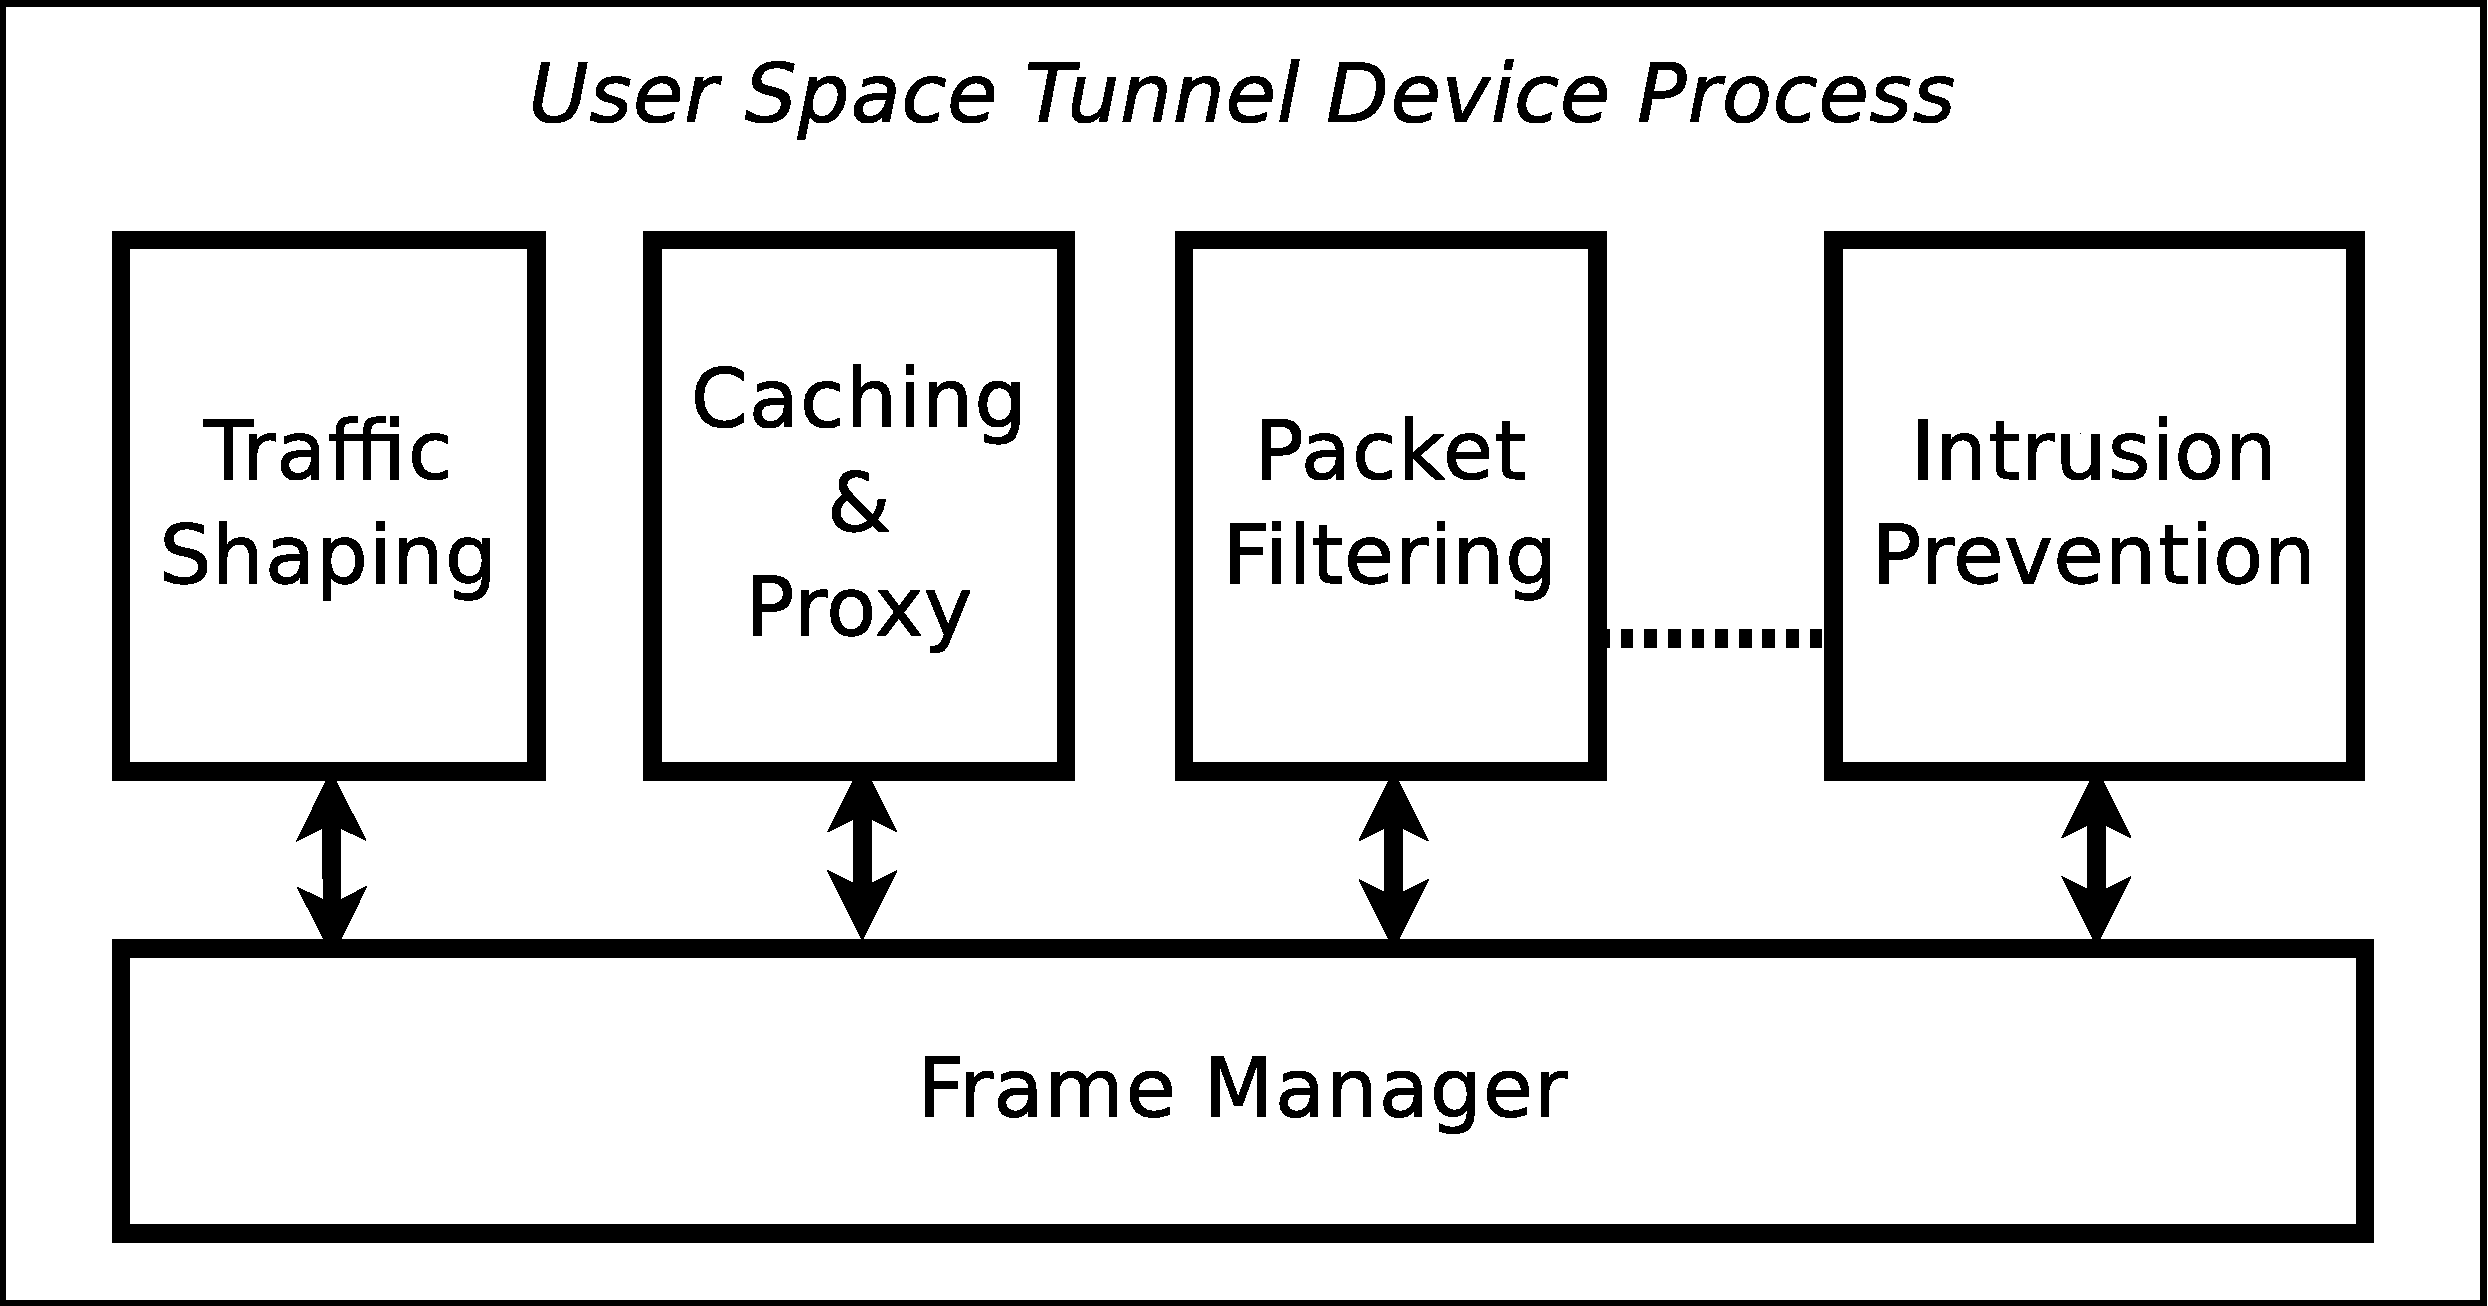
\includegraphics[width=0.6\columnwidth]{figures/TunProc.pdf}
%  \caption{Flow of packets in each \meddle}
%  \label{fig:MeddleboxPacketFlow}
% \end{figure}

\section{Overheads}

We now present the overheads incurred on tunnelling traffic through
\meddle.

\noindent\textbf{Power consumption.} We observed a 10\% increase in
power consumption when streaming an HD video from YouTube to an
Android device and an iPhone via one of our \meddle servers.  

\noindent\textbf{Data consumption.} IPsec encapsulation inflates
packet sizes, in addition to preventing carrier middleboxes from
applying their own compression. We measured the overhead of the 
tunnel in terms of data overhead from IPsec headers and keepalive
messages, finding that it ranges from 8--12\%. On each phone, an
Android phone and an iPhone, we accessed the Internet using the VPN
tunnel for one hour. Our test traffic included Web searches, map 
searches, online shopping, downloading popular apps, emailing and
reading the news. We also uploaded a picture to Facebook and Twitter, 
streamed a video on YouTube, and played a popular game (Angry Birds).

\noindent\textbf{Network Latency.} By forcing user traffic to \meddle 
and interposing on flows, we may add latency both due to additional
hops and due to processing time at the \meddle. We envision a
DONAR-style deployment where users are dynamically redirected to a
\meddle based on network conditions and server
load~\cite{wendell:donar}. Given this model, we evaluate whether we
can locate servers near mobile-network egress points using a
deployment such as PlanetLab, and found that this is generally the
case. For this experiment, we used data from approximately 10 mobile
phones located throughout the US and issued traceroutes from the
devices to targets in Google and Facebook's networks. We then used the
first non-private IP address seen from the mobile device on the path
to a server. We assume that this corresponds to the first router
adjacent to the mobile carrier's public Internet egress point. Using
this set of egress adjacencies, we determined the round-trip time from
each PlanetLab site, then took the average of the nearest five sites
to represent the case where a host at the nearest site is unavailable
due to load or other issues. The average latency to each router was
between 3\,ms and 13\,ms, with a median of 5\,ms. Thus, when compared
to RTTs of 10s or 100s of  milliseconds that exist in mobile networks,
the additional latencies from traversing a \meddle is expected to be
relatively small or even negligible. 

\section{Example Case Studies}

We believe that the research enabled by \meddle shall form a positive
feedback loop in which new, proven research artifacts become
additional incentives for user adoption, thus enabling further
research.   

For starters, we have implemented a DNS based filter to block ads,
analytics, and mediation sites. Blocking ads is an important incentive
because Vallina-rodriguez \etal~\cite{Vallina-rodriguez:2012:AdCache}
observe that ads account for 5\% of daily traffic from more than 50\%
of Android users in a large European ISP. Our ad blocking engine
relies on publicly available list of domains for ads and
analytics~\cite{YoyoAds}. We use the recent research on mobile
ads~\cite{Leontiadis:2012:AdsMobile, hornyack:appfence} to filter
domains specific to mobile networks.

\begin{table}
\centering
\begin{tabular}{|l|l|l|l|}
\hline
{\bf User} & {\bf Home (Wi-fi)} & {\bf Work (Wi-fi)} & {\bf Mobile (3G)} \\
\hline
User 1 & 84.4\% & 11.9\% & 3.7\% \\
\hline
User 2 & 95.1\% & 4.2\% & 0.7\% \\
\hline
\end{tabular}
\caption{Traffic volume from a mobile device when the user is either
  at home, or at work, or is mobile. \emph{A significant fraction of
    mobile traffic volume comes from Wi-fi networks.}}  
\label{tab:Usage}
\end{table}

In \fref{tab:Usage}, we summarize the traffic volume observed from two
users, one in the US and another in France. We observe that for these
two users the 3G traffic contributes to a very small fraction of the
total traffic from the mobile device. We are currently using our
\meddle system to validate similar results by an IRB approved study on
the network usage profiles of mobile phone users. 

\section{Future Work}

On each \meddle server, we plan on using Open
vSwitch~\cite{Openvswitch} to process packets on Virtual Machines
depending on the source of the traffic and the protocols used to
create the packets~\cite{Sekar:2012:ConsolidatedMBox}. This 
architecture enables us to test algorithms for content coalescing,
caching, prefetching, and offloading the work of processing the DOM to
speed up page load
times~\cite{silk,opera-mini,google-spdy}. Furthermore, we envision
that most of the interesting opportunities for mobile offloading will
come at the intersection of severe constraints for mobile devices
(power, data volume quota, and latencies) and the applications that
extensively exercise those constraints. For instance, distributed hash
tables (DHTs) are an example of a distributed service that has become
critical for a variety of applications from P2P communication to
content caching and anonymous networking. Using a split-application
model, mobile device need only send a request for a key to the
server-side and the server can perform all the network operations
required to locate the value without consuming mobile network
bandwidth. 

\scriptsize
\bibliographystyle{abbrv}
\bibliography{related_work}
\normalsize

\end{document}
